\chapter{Results and Discussion}\label{ch:4}

All four scenarios were executed end-to-end with the same orchestrator, the same tool layer and the same model endpoint (deepseek-V4.1-pro, served through an OpenAI-compatible interface). The complete suite takes about two minutes with a cold HTTP cache - almost all of it in the network-bound target-discovery stage; the other three scenarios run in seconds because their data are local (Table 9).

\section{Scenario 1: effector-target discovery in colorectal cancer}

DPEP1 is a GPI-anchored ectoenzyme: the UniProt entry (P16444, 411 aa) contains no transmembrane helix and no intracellular domain. The stage-1 audit therefore records a hard constraint - the effector cannot be DPEP1 itself, it must be a membrane protein able to transduce a signal - and immediately detects that the tool ocean contains no instrument for measuring signalling competence. The tool-creation agent builds one: a scorer combining UniProt topology, Pfam family, function annotation and localisation, with hard caps for GPI-anchored and secreted proteins. Its control set contains seven established receptors (LRP6 0.75, FZD1 0.85, EGFR 0.80, TNFRSF1A 0.85, TGFBR1 0.76, NOTCH1 0.68, IL6ST 0.73) and six non-signalling proteins (DPEP1 0.15, CEACAM5 0.15, ALB 0.12, INS 0.17, GAPDH 0.15, LYZ 0.12); all thirteen pass, the tool is registered, and stage 1 is re-run.

The candidate pool is built from four independent channels - STRING/IntAct partners (60), a 600-gene KEGG signalling panel screened for co-expression in TCGA-COADREAD (24 genes at |r| >= 0.30 and FDR <= 0.10), Reactome co-annotation (8 genes sharing a specific pathway) and PubMed co-mention - and filtered to 34 expressed candidates. The competence scorer reduces this to 10, and the six-dimension ranking produces Table 6.

\begin{table}[htbp]
\centering
\small
\caption{Six-dimension ranking for DPEP1 in colorectal cancer (run 20261116\_002640).}
\resizebox{\textwidth}{!}{%
\begin{tabular}{lccccccccc}
\hline
Rank & Gene & Composite & Assoc. & Signal. & Disease & Pathway & Novelty & Drug. & Dims >= 0.6 \\
\hline
1 & ASIC1 & 0.496 & 0.42 & 0.69 & 0.41 & 0.04 & 0.57 & 0.72 & 2/6 \\
2 & NOTCH1 & 0.481 & 0.51 & 0.68 & 0.36 & 0.00 & 0.03 & 0.92 & 2/6 \\
3 & FZD7 & 0.459 & 0.23 & 0.85 & 0.23 & 0.23 & 0.30 & 0.84 & 2/6 \\
4 & ZNRF3 & 0.449 & 0.50 & 0.75 & 0.49 & 0.00 & 0.41 & 0.25 & 1/6 \\
5 & ACE2 & 0.443 & 0.61 & 0.45 & 0.20 & 0.02 & 0.03 & 1.00 & 2/6 \\
\hline
\end{tabular}
}
\end{table}

Three observations matter more than the ordering. First, the top four candidates are all signal-transducing membrane proteins that are co-expressed with DPEP1 in CRC - the acid-sensing ion channel ASIC1, NOTCH1 (r = +0.44), ZNRF3 (r = +0.43) and the Wnt receptor FZD7 - which is exactly the biological class the topological constraint predicts. Second, the scores are close: the top five span only 0.053, so the system reports a prioritisation rather than a decision, and the report states this explicitly. Third, no candidate reaches three strong dimensions, because association with a GPI-anchored protein is intrinsically hard to establish from public data; the critic logs this as a failed check instead of hiding it (Figure 3).

\begin{figure}[htbp]
\centering
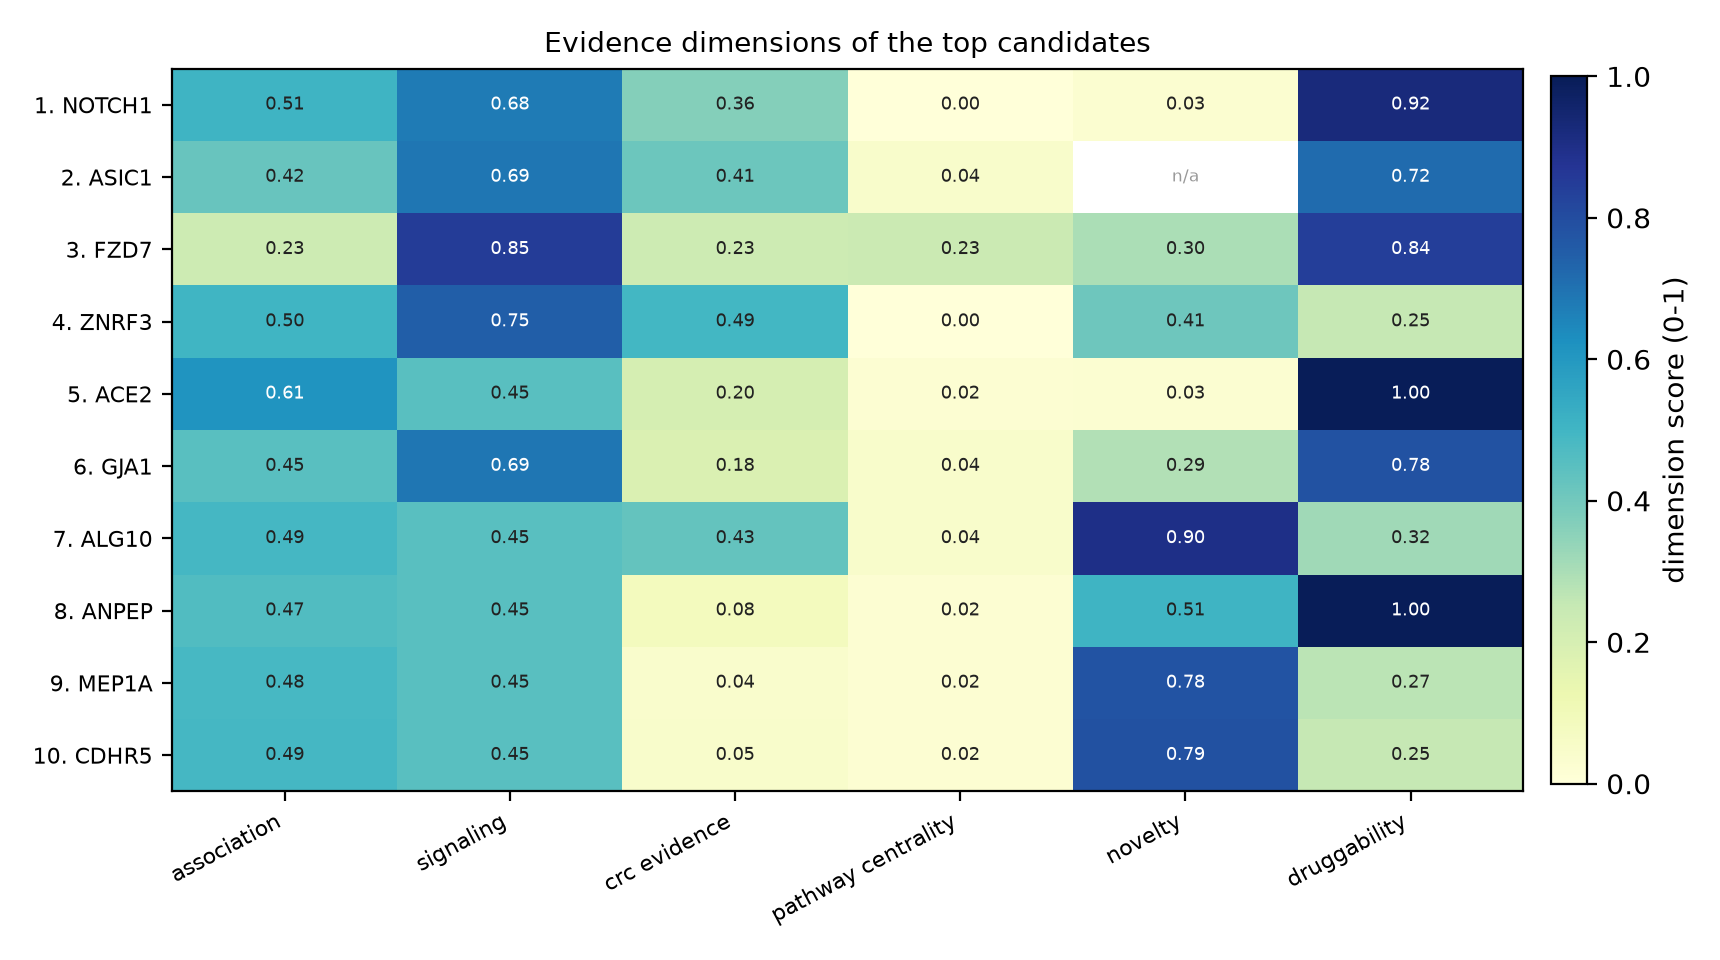
\includegraphics[width=0.99\textwidth]{figures/fig_target_heatmap.png}
\caption{Dimension scores of the top ten candidates. The block structure shows where each candidate draws its support: NOTCH1 and ASIC1 on signalling and druggability, ZNRF3 on association and signalling, ACE2 on association alone.}
\end{figure}

\section{Hindcast: does MOCHI recover the published effector LRP6?}

The Wnt co-receptor LRP6 is the effector reported in the experimental study that motivated this project. It is therefore a natural hidden test. Without any prior, LRP6 is not nominated at all: in TCGA-COADREAD its expression is essentially uncorrelated with DPEP1 (r = -0.084), it has no STRING or IntAct interaction with DPEP1, and the two proteins share no specific Reactome pathway. Nomination would require prior knowledge, not more data.

We therefore ran the same pipeline with LRP6 injected as a hypothesis seed (the -{}-seed-genes mode) so that it is scored on identical terms. LRP6 obtains the highest competence tier (0.754) but the lowest association (0.098) and low novelty (0.142, because it is heavily studied); its composite score is 0.306 and it ranks 11th of 11 (Table 7). This is the correct behaviour for an evidence-driven system: it does not manufacture support for a hypothesis that the data do not contain. The result also separates the two questions a reviewer should ask - 'is LRP6 a competent effector?' (yes) and 'is it supported as the effector of DPEP1 in this cohort?' (no) - which is precisely the distinction the dossier reports.

\begin{table}[htbp]
\centering
\small
\caption{LRP6 hindcast. Data-driven channels do not nominate LRP6; when scored as a hypothesis it is competent but poorly associated.}
\resizebox{\textwidth}{!}{%
\begin{tabular}{lcccccc}
\hline
Gene & Nominated by data & Competence & Association & Novelty & Composite & Rank \\
\hline
LRP6 (no seed) & no & - & - & - & - & - \\
LRP6 (seeded) & prior & 0.754 & 0.098 & 0.142 & 0.306 & 11/11 \\
\hline
\end{tabular}
}
\end{table}

\subsection{From a receptor-class shortlist to a validated target}

The shortlist and the validated target answer different questions, and the project is strongest when it keeps them apart. The unbiased screen answers 'which membrane receptors could relay a GPI-anchored ectoenzyme in CRC?' and returns the Wnt/Notch co-receptor class (NOTCH1, ZNRF3, FZD7) together with a druggable ion channel (ASIC1). It does not, and cannot from these cohorts, answer 'is LRP6 the relay for DPEP1?' - because that question requires physical and perturbation evidence that public co-expression data do not contain.

That is why the programme did not stop at the ranking. Guided by the Wnt/Notch shortlist, the experimental collaborators tested LRP6 directly: reciprocal co-im\-mu\-no\-pre\-cip\-i\-ta\-tion established that DPEP1 and LRP6 associate in CRC cells; knockdown and overexpression showed that the DPEP1-driven phenotype depends on LRP6; qPCR and Western blot readouts placed the effect on the Wnt output; and site-directed mutagenesis of the predicted interface identified the residues required for the dependency. The computational stage contributed the receptor class, the mechanistic hypothesis and - critically - an explicit statement of the missing evidence, which is what made the IP experiment the obvious next step rather than a fishing expedition.

Reporting the negative result is therefore not a weakness of the demo but the part that makes it useful: the system quantified exactly which link was unproven (association, 0.098) while asserting which link was plausible (competence, 0.754), and the wet lab resolved the former. A system that had ranked LRP6 first on the strength of co-expression alone would have been right for the wrong reason.

\section{Scenario 2: structure- and prior-guided enzyme design}

Strictosidine synthase (P68175, 344 aa) catalyses the Pictet-Spengler condensation of tryp\-ta\-mine and se\-co\-lo\-ga\-nin. A published round-1 scan identified M276 as a productive position and three positions (G210, H307, P253) as dead zones; a round-2 library then found M276L (+2.1x), V176F (+1.5x), E306S/T (-64\% to -75\%) and confirmed G210S as dead. We gave MOCHI only the sequence, an AlphaFold model and the round-1 outcomes, and asked for a 15-variant library.

The structural stage places 154 positions within 12 A of the catalytic cluster and enumerates 2,773 single substitutions. The top of the designed library is shown in Table 8: M276L is ranked first of 2,773, and the library covers 12 distinct positions with at most two substitutions per position. Every variant carries a QuikChange primer pair designed from the native CDS (ENA Y00756, mapped by translated-frame alignment): for M276L the codon changes ATG -> CTG and the forward primer is 5'-GAATTAGATGGAAATCTGCACGGAAGAGTTGAT-3' (T\_m 60.7 C, GC 39.4\%). Figure 4A shows the same ranking graphically.

\begin{table}[htbp]
\centering
\small
\caption{Top of the designed round-2 library. 'Prior' is the round-1 outcome for that position.}
\resizebox{\textwidth}{!}{%
\begin{tabular}{lcccccccc}
\hline
Rank & Variant & d to site (A) & Leverage & Chemistry & Prior & Packing & Score & Published outcome \\
\hline
1 & M276L & 1.34 & 0.89 & 0.50 & hit & 0.97 & 0.601 & hit (+2.1x) \\
2 & M276I & 1.34 & 0.89 & 0.42 & hit & 0.97 & 0.561 & not tested \\
3 & Q310E & 1.34 & 0.89 & 0.50 & untested & 0.94 & 0.432 & not tested \\
4 & E306Q & 1.33 & 0.90 & 0.50 & reduced & 0.94 & 0.420 & not tested \\
5 & Y105F & 3.24 & 0.76 & 0.58 & untested & 0.96 & 0.404 & not tested \\
6 & E306D & 1.33 & 0.90 & 0.50 & reduced & 0.70 & 0.388 & not tested \\
7 & A152S & 1.34 & 0.89 & 0.42 & untested & 1.00 & 0.386 & not tested \\
\hline
\end{tabular}
}
\end{table}

Hindcast performance is mixed in a way that is informative. At variant level the system recovers 1 of 2 active variants (M276L, rank 1 of 2,773); at position level it recovers 1 of 2 positions; and it excludes 3 of 3 experimentally dead positions. The miss is V176F (global rank 2,004), a second-shell aromatic substitution 7.7 A from the catalytic cluster whose benefit comes from packing against the substrate rather than from proximity to the active site. A distance-and-conservation model cannot see that effect; an energy model (FoldX, Rosetta) or a learned mutation predictor would be required. The system reports the miss rather than hiding it, and the report names the missing capability - which is exactly the behaviour the tool-creation loop is designed to trigger in a future run.

The prior ablation isolates the contribution of experimental knowledge. With the round-1 prior, M276L ranks first; without it, the same variant falls to fourth, because a neighbouring untested position with a conservative substitution overtakes it. Dead-zone exclusion, by contrast, survives without the prior: the buried-glycine penalty in the packing term removes G210 substitutions on structural grounds alone. The two sources of knowledge are therefore complementary rather than redundant.

\section{Scenario 3: multi-step retrosynthesis of a hindered local anaesthetic}

We replaced the textbook aspirin example with lidocaine, a blockbuster local anaesthetic whose synthesis is short but not trivial: the molecule contains a sterically hindered 2,6-dimethylanilide, a tertiary amine and a glycine linker, and a naive planner will either stop at a non-purchasable acid or acylate the wrong nitrogen. The target has two obvious amide bonds and one N-alkylation site, so the order of disconnection matters.

MOCHI plans a two-step route that matches the step count of the industrial process. The first disconnection is the amide, giving 2,6-di\-methyl\-an\-i\-line and N,N-di\-ethyl\-gly\-cine; because that glycine is a specialty reagent rather than a standard building block, it is absent from the curated stock, so the planner cannot stop there and is forced to expand it. The second disconnection is an N-alkylation that delivers diethylamine and bromoacetic acid, both purchasable. The route is therefore complete, uses two different reaction classes, and every leaf is a real catalogue compound (Table 9).

Two details make this a better demonstration than a one-step esterification. First, the chemo\-se\-lec\-tiv\-ity problem is explicit in the route: the amide nitrogen is acylated while the tertiary amine is alkylated, which is the order the industrial synthesis uses. Second, the planner had to recognise that a plausible looking acyl fragment is not itself a building block - the same failure mode that defeats naive template planners on real targets.

\begin{table}[htbp]
\centering
\small
\caption{Retrosynthesis benchmark. Every target is solved, and no planned route is longer than its literature counterpart.}
\begin{tabularx}{\textwidth}{l>{\raggedright\arraybackslash}X>{\raggedright\arraybackslash}X>{\raggedright\arraybackslash}X>{\raggedright\arraybackslash}X}
\hline
Drug & Literature steps & Planned steps & Solved & Confidence \\
\hline
Lidocaine & 2 & 2 & yes & 0.66 \\
Phenacetin & 2 & 2 & yes & 0.66 \\
Benorilate & 3 & 3 & yes & 0.54 \\
Sulfanilamide & 2 & 2 & yes & 0.66 \\
Aspirin & 1 & 1 & yes & 0.83 \\
Paracetamol & 1 & 1 & yes & 0.83 \\
Benzocaine & 1 & 1 & yes & 0.83 \\
Vanillin & 2 & 1 & yes & 0.83 \\
\hline
\end{tabularx}

\end{table}

The same run also plans the three-step synthesis of ben\-or\-i\-late (Benoral), and the route is instructive: the ester disconnection splits the molecule into acetylsalicylic acid and paracetamol, each of which is itself a drug that the planner then disconnects to simple building blocks. In other words the search recovers the fact that ben\-or\-i\-late is a mutual prodrug, without being told. Across the eight-drug suite the planner solves every target with a mean of 1.62 planned steps against 1.75 literature steps (Table 9 and Figure 4B). The suite is deliberately restricted to targets whose syntheses stay inside the six reaction classes of the template set; epoxide opening, Friedel-Crafts acylation and similar transformations are out of scope and are the natural next addition to the tool layer.

\section{Scenario 4: compiling protocols into SDL instructions}

The stric\-to\-si\-dine-synthase activity assay is compiled into six opcodes - TRANSFER, TRANSFER, INCUBATE, TRANSFER, CENTRIFUGE, MEASURE - with volumes in millilitres, a 30 C incubation for 30 min, and a 48-minute simulated timeline whose bottleneck is the incubator (Figure 4C). The compiler flags four defaults (steps without an explicit duration), all of which are reported rather than silently applied.

The benchmark is the more informative test. Six clean protocols are all accepted by the validator, and five deliberately corrupted protocols are all caught (Table 10): a 5 mL aliquot in a 2 mL vial (vessel overflow), a 300 C set-point on a 150 C block, diethyl ether heated above its flash point, a quench with no stated volume, and a zero-minute incubation. The flammable-solvent case is the most interesting, because the hazard is not local to one sentence: the solvent appears in step 1 and the temperature in step 2, so the validator screens the protocol as a whole.

\begin{table}[htbp]
\centering
\small
\caption{Protocol compiler benchmark: 6/6 clean protocols valid, 5/5 corrupted protocols caught.}
\resizebox{\textwidth}{!}{%
\begin{tabular}{lccccc}
\hline
Protocol & Steps & Opcodes & Injected fault & Detected & Caught \\
\hline
STR activity assay & 6 & 6 & - & - & n/a \\
Suzuki coupling & 7 & 7 & - & - & n/a \\
HATU amide coupling & 6 & 6 & - & - & n/a \\
Reductive amination & 6 & 6 & - & - & n/a \\
Recrystallisation & 5 & 5 & - & - & n/a \\
HPLC sample prep & 5 & 5 & - & - & n/a \\
Oversized aliquot & 4 & 4 & vessel\_overflow & vessel\_overflow & yes \\
Impossible temperature & 3 & 3 & temperature\_limit & temperature\_limit & yes \\
Flammable solvent & 3 & 3 & flammable\_hazard & flammable\_hazard & yes \\
Missing volume & 4 & 4 & missing\_volume & missing\_volume & yes \\
Zero duration & 3 & 3 & non\_positive\_duration & non\_positive\_duration & yes \\
\hline
\end{tabular}
}
\end{table}

\begin{figure}[htbp]
\centering
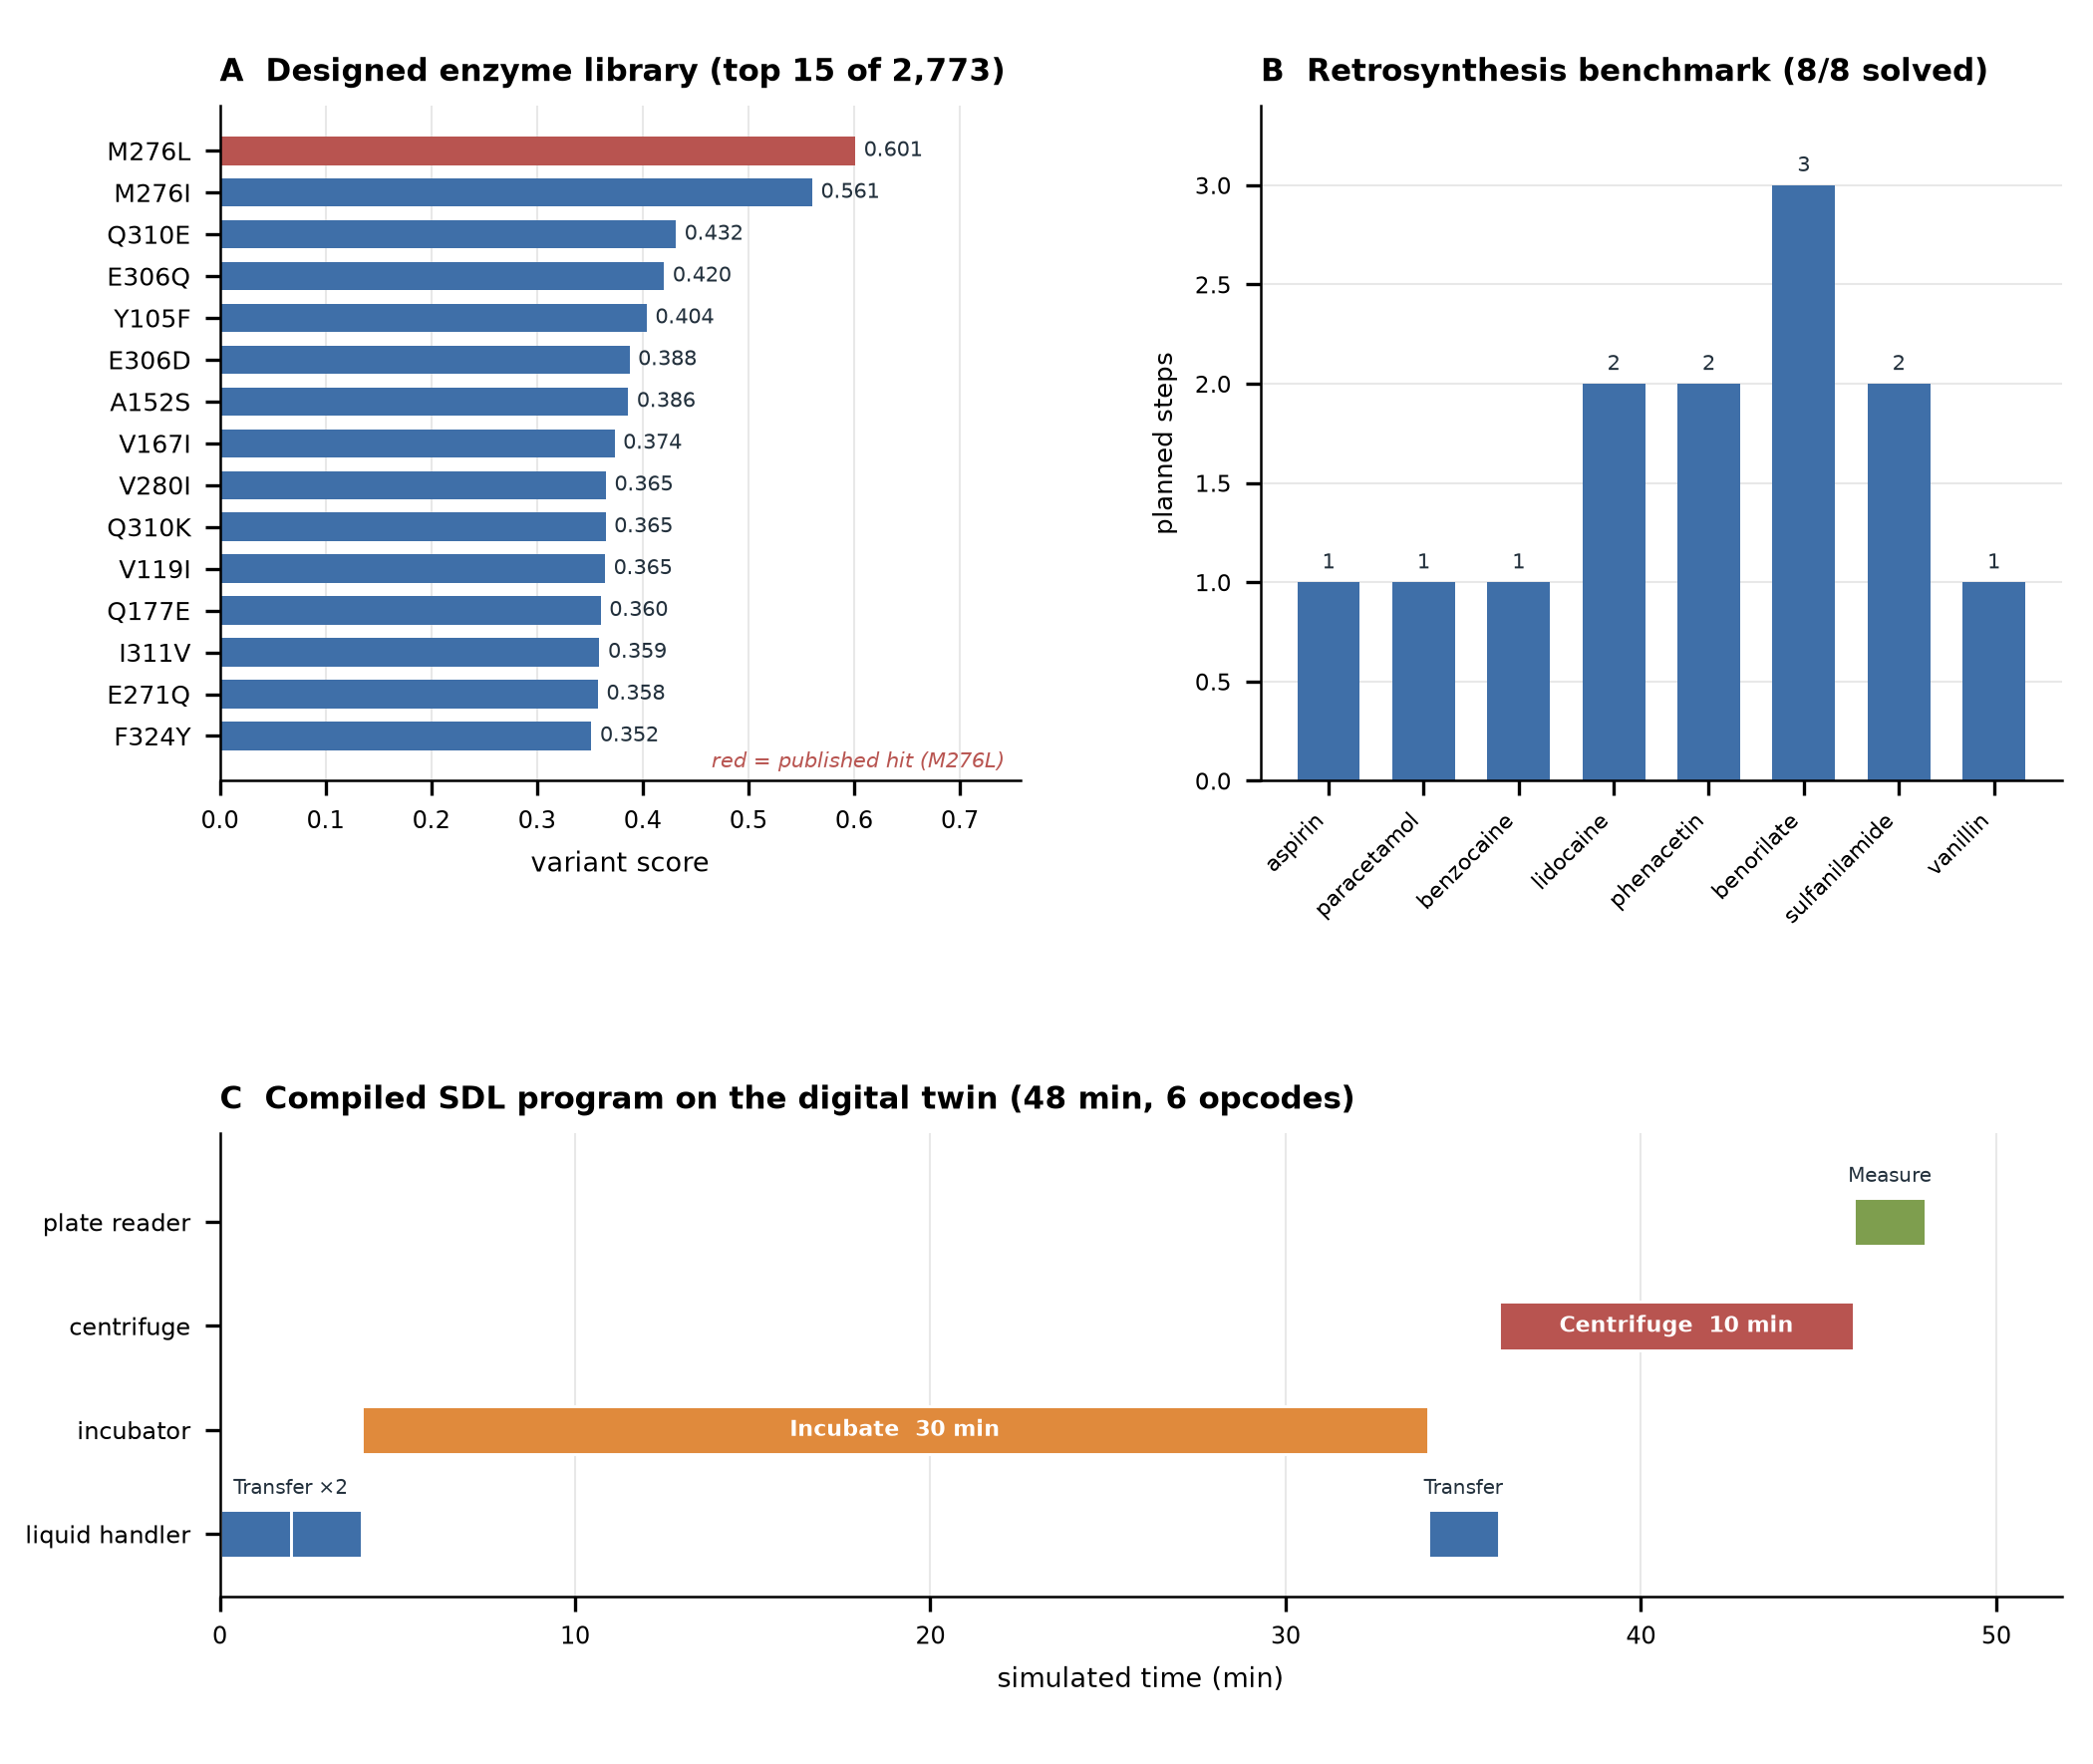
\includegraphics[width=0.99\textwidth]{figures/fig_panels.png}
\caption{Results of the three computational scenarios. (A) Designed enzyme library: the top 15 of 2,773 scored variants; the published hit M276L ranks first (red). (B) Retrosynthesis benchmark: planned step count per drug; the two unsolved targets are shown in grey. (C) Compiled SDL program on the digital twin: every opcode is placed on its device and on the simulated timeline (48 min, 6 opcodes).}
\end{figure}

\section{Ablations}

Two ablations test the two mechanisms that distinguish MOCHI from a simple tool-calling loop (Table 11). Disabling runtime tool creation leaves the target-discovery pipeline unable to enforce the effector constraint: stage 3 reports the capability gap, the critic raises it, but no tool is built, and stage 4 has zero candidates. Disabling the experimental prior leaves the enzyme scorer functional but degrades the top of the ranking, moving the true best variant from rank 1 to rank 4. Both mechanisms are therefore load-bearing rather than decorative.

\begin{table}[htbp]
\centering
\small
\caption{Ablations. Removing either mechanism removes a capability, not just a few points.}
\begin{tabularx}{\textwidth}{l>{\raggedright\arraybackslash}X>{\raggedright\arraybackslash}X>{\raggedright\arraybackslash}X}
\hline
Configuration & Stage 3 & Stage 4 & Key metric \\
\hline
Full pipeline (S1) & ok (10 competent) & 10 ranked & top-1 ASIC1, 0.496 \\
No tool creation (S1) & failed (capability gap) & 0 ranked & no ranking produced \\
Full pipeline (S2) & 2773 scored & 15 designed & M276L rank 1/2773 \\
No experimental prior (S2) & 2773 scored & 15 designed & M276L rank 4/2773 \\
\hline
\end{tabularx}

\end{table}

\section{Runtime, stability and discussion}

\begin{table}[htbp]
\centering
\small
\caption{Runtime of the four scenarios under the same orchestrator and model endpoint.}
\begin{tabularx}{\textwidth}{l>{\raggedright\arraybackslash}X>{\raggedright\arraybackslash}X>{\raggedright\arraybackslash}X>{\raggedright\arraybackslash}X}
\hline
Scenario & Wall time & Stages ok & Tool calls & Reproducible offline \\
\hline
S1 target discovery & 120 s cold / 19 s warm & 4/4 & > 200 & yes (cached) \\
S2 enzyme design & 6.2 s / 2.1 s & 4/4 & 6 & yes \\
S3 retrosynthesis & 0.3 s & 4/4 & \textasciitilde{}20 & yes \\
S4 protocol $\rightarrow$ SDL & 0.2 s & 4/4 & \textasciitilde{}30 & yes \\
\hline
\end{tabularx}

\end{table}

Two stability observations are worth reporting. First, the identity of the top four targets is stable across repeated runs, while their order changes by less than 0.02 when the critic re-calibrates weights from dimension coverage; this is exactly the uncertainty the report quantifies, and is why the system reports a confidence band rather than a single winner. Second, determinism is a property of the data plane, not of the model: re-running with a different engine changes the prose but not the numbers, because every number is computed in Python from cached, hashed responses.

The main limitation is coverage. The co-expression screen uses a 600-gene KEGG signalling panel rather than the whole transcriptome, the enzyme scorer is a physics-light heuristic, the retrosynthesis template set is deliberately small, and the protocol parser handles the imperative style of standard SOPs rather than arbitrary prose. Each limitation is a place where the framework's own tool-creation loop could be pointed next - and, in the target scenario, already was.

